
\section{Experiences With Coordination}
\label{sec:evaluation}

When achievable, coordination-free execution enables scalability
limited to that of available hardware. This is powerful: an
\iconfluent application can scale out without
sacrificing correctness, latency, or availability. In
Section~\ref{sec:bcc-practice}, we saw combinations of invariants
and transactions that were \iconfluent and others that were not. In this
section, we apply these combinations to the workloads of the
OLTP-Bench suite~\cite{oltpbench}, with a focus on the TPC-C
benchmark. Our focus is on the coordinaton required in order to
correctly execute each and the resulting, coordination-related
performance costs.

\subsection{TPC-C Invariants and Execution}
\label{sec:tpcc-invariants}

The TPC-C benchmark is the gold standard for database concurrency
control~\cite{oltpbench} both in research and in industry~\cite{tpcc},
and in recent years has been used as a yardstick for distributed
database concurrency control
performance~\cite{calvin,hstore,silo}. How much coordination does
TPC-C actually require a compliant execution?

The TPC-C workload is designed to be representative of a wholesale
supplier's transaction processing requirements. The workload has a number of
application-level correctness criteria that represent basic business
needs (e.g., order IDs must be unique) as formulated by the TPC-C
Council and which must be maintained in a compliant run. We can
interpret these well-defined ``consistency criteria'' as invariants and
subsequently use \iconfluence analysis to determine which transactions
require coordination and which do not.

Table~\ref{table:tpcc-invariants} summarizes the twelve invariants
found in TPC-C as well as their \iconfluence analysis results as
determined by Table~\ref{table:invariants}. We classify the invariants
into three broad categories: materialized view maintenance, foreign
key constraint maintenance, and unique ID assignment. As we discussed
in Section~\ref{sec:bcc-practice}, the first two categories are
\iconfluent (and therefore maintainable without coordination) because
they only regulate the \textit{visibility} of updates to multiple
records. Because these (10 of 12) invariants are \iconfluent under the
workload transactions, there exists some execution strategy that does
not use coordination. However, simply because these invariants are
\iconfluent does not mean that \textit{all} execution strategies will
scale well: for example, using locking would \textit{not} be
coordination-free.


\begin{table}[t!]
\definecolor{yesgray}{gray}{0.92}
\small
\begin{tabular}{|l|l|l|l|l|}
  \hline
  \textbf{\#} & \textbf{Informal Invariant Description} &
  \textbf{Type} & 
  \textbf{Txns} & \textbf{$\mathcal{I}$-C} \\\hline
  \rowcolor{yesgray}
  1 & {\scriptsize YTD wh sales = sum(YTD district sales)} & MV &
  P & Yes\\
  2 &  {\scriptsize Per-district order IDs are sequential} &$\mathrm{S_{ID}}$+FK  & N, D & No\\
  3 &  {\scriptsize New order IDs are sequentially assigned} & $\mathrm{S_{ID}}$  & N, D & No \\
  \rowcolor{yesgray}
  4 & {\scriptsize  Per-district, item order count = roll-up} & MV &
  N & Yes\\
  \rowcolor{yesgray}
  5 &  {\scriptsize Order carrier is set iff order is pending} & FK &
  N, D & Yes \\
  \rowcolor{yesgray}
  6 &  {\scriptsize Per-order item count = line item roll-up} & MV & N
  & Yes \\
  \rowcolor{yesgray}
  7 &  {\scriptsize Delivery date set iff carrier ID set} & FK & D & Yes \\
  \rowcolor{yesgray}
  8 &  {\scriptsize YTD wh = sum(historical wh)} & MV &
  D & Yes \\
  \rowcolor{yesgray}
  9 &  {\scriptsize YTD district = sum(historical district)} &
  MV & P & Yes \\
  \rowcolor{yesgray}
  10 &  {\scriptsize Customer balance matches expenditures} & MV & P, D & Yes \\
  \rowcolor{yesgray}
  11 &  {\scriptsize Orders reference New-Orders table}  & FK & N & Yes \\
  \rowcolor{yesgray}
  12 &  {\scriptsize Per-customer balance = cust. expenditures} & MV & P, D &
  Yes \\\hline

\end{tabular}
\caption{TPC-C Declared ``Consistency Conditions'' (3.3.2.x) and \iconfluence
  analysis results
  (Invariant type: MV: materialized view, $\mathbf{S_{ID}}$: sequential ID assignment, FK: foreign
  key; Transactions: N: New-Order, P: Payment, D: Delivery).}
\label{table:tpcc-invariants}
\end{table}


As one coordination-free execution strategy (which we implement in
Section~\ref{sec:evaltpcc}) that respects the foreign key and
materialized view invariants, we can use RAMP transactions, which
provide atomically visible transactional updates across servers
without relying on coordination for correctness~\cite{ramp-txns}. In
brief, RAMP transactions employ limited multi-versioning and metadata
to ensure that readers and writers can always proceed concurrently:
any client whose reads overlap with another client's writes to the
same item(s) can use metadata stored in the items to fetch any
``missing'' writes from the respective servers. A standard RAMP
transaction over data items suffices to enforce foreign key
constraints, while a RAMP transaction over commutative counters as
described in~\cite{ramp-txns} is sufficient to enforce the TPC-C
materialized view constraints.

Two of TPC-C's invariants are not \iconfluent with respect to the
workload transactions and therefore \textit{do} require
coordination. On a per-district basis, order IDs should be assigned
sequentially (both uniquely and sequentially, in the New-Order
transaction) and orders should be processed sequentially (in the
Delivery transaction). If the database is partitioned by warehouse (as
is standard~\cite{silo,calvin,hstore}), the former is a distributed
transaction (by default, $10\%$ of New-Order transactions span
multiple warehouses). The benchmark specification allows the latter to
be run asynchronously and in batch mode on a per-warehouse
(non-distributed) basis, so we, like others~\cite{calvin,silo}, focus
on New-Order. Including additional transactions like the read-only
Order-Status in the workload mix would increase performance due to the
transactions' lack of distributed coordination and (often
considerably) smaller read/write footprints.

\minihead{Avoiding New-Order Coordination} New-Order is not
\iconfluent with respect to the TPC-C invariants, so we can always
fall back to using serializable isolation. However, the per-district
ID assignment records (10 per warehouse) would become a point of contention,
limiting our throughput to effectively $\frac{100W}{RTT}$ for a
$W$-warehouse TPC-C benchmark with the expected $10\%$ distributed
transactions. Others~\cite{silo} (including us, in prior
work~\cite{hat-vldb}) have suggested disregarding consistency criteria
3.3.2.3 and 3.3.2.4, instead opting for unique but non-sequential ID
assignment: this allows inconsistency and violates the benchmark
compliance criteria.

During a compliant run, New-Order transactions must
coordinate. However, as discussed above, only the ID assignment
operation is non-I-confluent; the remainder of the operations in the
transaction can execute coordination-free. With some effort, we can
avoid distributed coordination. A na\"{\i}ve implementation might grab
a lock on the appropriate district's ``next ID'' record, perform
(possibly remote) remaining reads and writes, then release the lock at
commit time. Instead, as a more efficient solution, New-Order can
defer ID assignment until commit time by introducing a layer of
indirection. New-Order transactions can generate a temporary, unique,
but non-sequential ID (\texttt{tmpID}) and perform updates using this
ID using a RAMP transaction (which, in turn, handles the foreign key
constraints)~\cite{ramp-txns}. Immediately prior to transaction
commit, the New-Order transaction can assign a ``real'' ID by
atomically incrementing the current district's``next ID'' record
(yielding \texttt{realID}) and recording the \texttt{[tmpID, realID]}
mapping in a special ID lookup table. Any read requests for the
\texttt{ID} column of the Order, New-Order, or Order-Line tables can
be safely satisfied (transparently to the end user) by joining with
the ID lookup table on \texttt{tmpID}. In effect, the New-Order ID
assignment can use a nested atomic
transaction~\cite{atomictransactions} upon commit, and all
coordination between any two transactions is confined to a
single server.

\subsection{Evaluating TPC-C New-Order}
\label{sec:evaltpcc}


\begin{figure}
\hspace{1.5em}
\includegraphics{figs/ca_serial_legend.pdf}\vspace{-1em}
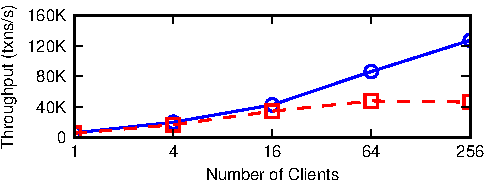
\includegraphics[width=\columnwidth]{figs/client_thru.pdf}
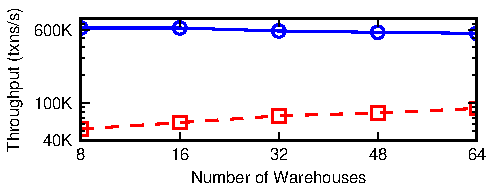
\includegraphics[width=\columnwidth]{figs/wh_thru.pdf}
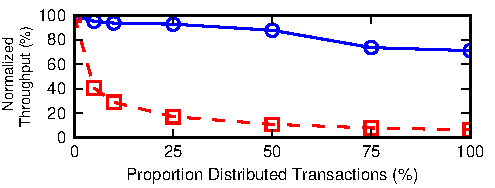
\includegraphics[width=\columnwidth]{figs/remote_thru.pdf}\vspace{-.5em}
%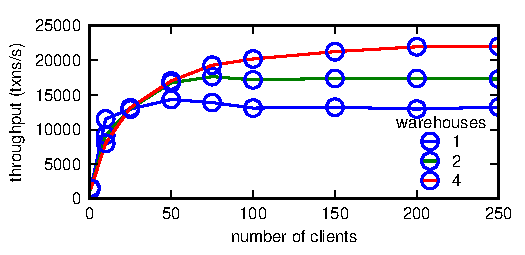
\includegraphics[width=\columnwidth]{figs/wh_thru_single.pdf}
\caption{TPC-C New-Order throughput across eight servers.}
\label{fig:clients}
\end{figure}


We subsequently implemented the above execution strategy in a distributed
database prototype to quantify the overheads associated with
coordination in TPC-C New-Order. In brief, the coordination-avoiding
query plan scales linearly to over 12.7M transactions per second on
$200$ servers while substantially outperforming distributed two-phase
locking. Our goal here is to demonstrate---beyond the microbenchmarks of
Section~\ref{sec:motivation}---that safe but judicious use of
coordination can have meaningful positive effect on performance.

\begin{comment}
We originally ported TPC-C
New-Order to our prior RAMP transaction prototype~\cite{ramp-txns} but
found that the larger transaction footprint was poorly suited for the
threading model. Each New-Order transaction generates between 13--33
reads and 13--33 writes, so switching to an event-based RPC layer with
support for batching and connection pooling delivered an approximate
factor of two improvement in throughput, while additional optimization
(e.g., more efficient indexing, fewer object allocations) delivered
another factor of two. 
\end{comment}

\minihead{Implementation and Deployment} We employ a multi-versioned
storage manager, with RAMP-Fast transactions for snapshot reads and
atomically visible writes/``merge'' (providing a variant of regular
register semantics, with writes visible to later transactions after
commit)~\cite{ramp-txns} and implement the nested atomic transaction
for ID assignment as a sub-procedure inside RAMP-Fast's server-side
commit procedure (using spinlocks). We implement transactions as
stored procedures and fulfill the TPC-C ``Isolation Requirements'' by
using read and write buffering as proposed in~\cite{hat-vldb}. As is
common~\cite{calvin,abadi-vll,hstore,jones-dtxn}, we disregard
per-warehouse client limits and ``think time'' to increase load per
warehouse. In all, our base prototype architecture is similar to that
of~\cite{ramp-txns}: a JVM-based partitioned, main-memory, mastered
database.

For an apples-to-apples comparison with a coordination-intensive
technique within the same system, we also implemented textbook
two-phase locking (2PL)~\cite{bernstein-book}, which provides
serializability but also requires distributed coordination. We totally
order lock requests across servers to avoid deadlock, batching lock
requests to each server and piggybacking read and write requests on
lock request RPC. As a validation of our implementation, our 2PL
prototype achieves per-warehouse (and sometimes aggregate) throughput
similar to (and often in excess of) several recent serializable
database implementations (of both 2PL and other
approaches)~\cite{calvin,abadi-vll,hstore,jones-dtxn}.

By default, we deploy our prototype on eight EC2 \texttt{cr1.8xlarge}
instances in the Amazon EC2 \texttt{us-west-2} region (with
non-co-located clients) with one warehouse per server (recall there
are 10 ``hot'' district ID records per warehouse) and report the
average of three 120 second runs.

\minihead{Basic behavior} Figure~\ref{fig:clients} shows performance
across a variety of configurations, which we detail below. Overall,
the coordination-avoiding query plan far outperforms the serializable
execution. The coordination-avoiding query plan performs some
coordination, but, because coordination points are not distributed
(unlike 2PL), physical resources (and not coordination) are the bottleneck.

\miniheadit{Varying load} As we increase the number of clients, the
coordination-avoiding query plan throughput increases linearly, while
2PL throughput increases to $40$K transactions per second, then levels
off. As in our microbenchmarks in Section~\ref{sec:motivation}, the
former utilizes available hardware resources (bottlenecking
on CPU cycles at $640$K transactions per second), while the latter
bottlenecks on logical contention.

\miniheadit{Physical resource consumption} To understand the overheads
of each component in the coordination-avoiding query plan, we used JVM
profiling tools to sample thread execution while running at peak
throughput, attributing time spent in functions to relevant modules
within the database implementation (where possible):

\vspace{-.5em}
\begin{center}
\centering
\small
\setlength{\fboxsep}{4pt}
\fbox{
\begin{tabular}{l r}
\textbf{Code Path} & \textbf{Cycles}\\
Storage Manager (Insert, Update, Read) & 45.3\%\\
Stored Procedure Execution & 14.4\%\\
RPC and Networking & 13.2\%\\
Serialization & 12.6\%\\
ID Assignment Synchronization (spinlock contention) & 0.19\%\\
Other & 14.3\%\\
\end{tabular}}
\end{center}
\vspace{-.5em}

The coordination-avoiding prototype spends a large portion of
execution in the storage manager, performing B-tree modifications and
lookups and result set creation, and in RPC/serialization. In contrast
to 2PL, the prototype spends less than $0.2\%$ of time coordinating,
in the form of waiting for locks in the New-Order ID assignment; the
(single-site) assignment is fast (a linearizable integer increment and
store, followed by a write and fence instruction on the spinlock), so
this should not be surprising. We observed large throughput penalties
due to garbage collection (GC) overheads (up to 40\%)---an unfortunate
cost of our highly compact (several thousand lines of Scala),
JVM-based implementation. However, even in this current prototype,
physical resources are the bottleneck---not coordination.

\miniheadit{Varying contention} We subsequently varied the number of
``hot,'' or contended items by increasing the number of warehouses on
each server. Unsurprisingly, 2PL benefits from a decreased
contention, rising to over $87$K transactions per second with $64$
warehouses. In contrast, our coordination-avoiding implementation is
largely unaffected (and, at $64$ warehouses, is even negatively
impacted by increased GC pressure). The coordination-avoiding query
plan is effectively agnostic to read/write contention.

\miniheadit{Varying distribution} We also varied the percentage of
distributed transactions. The coordination-avoiding query plan
incurred a $29\%$ overhead moving from no distributed transactions to
all distributed transactions due to increased serialization overheads
and less efficient batching of RPCs. However, the 2PL implementation decreased in throughput by over $90\%$ (in line
with prior results~\cite{abadi-vll,calvin}, albeit exaggerated here
due to higher contention) as more requests stalled due to coordination
with remote servers.

\minihead{Scaling out} Finally, we examined our prototype's scalability,
again deploying one warehouse per server. As Figure~\ref{fig:scaleout}
demonstrates, our prototype scales linearly, to over 12.74 million
transactions per second on 200 servers (in light of our earlier
results, and, for economic reasons, we do not run 2PL at this
scale). Per-server throughput is largely constant after 100 servers,
at which point our deployment spanned all three \texttt{us-west-2}
datacenters and experienced slightly degraded per-server performance.
While we make use of application semantics, we are unaware of
any other compliant multi-server TPC-C implementation that has
achieved greater than 500K New-Order transactions per
second~\cite{calvin,jones-dtxn,hstore,abadi-vll}.

\minihead{Summary} We present these quantitative results as a proof of
concept that executing even challenging workloads like TPC-C that
contain complex integrity constraints are not necessarily at odds with
scalability if implemented in a coordination-avoiding
manner. Distributed coordination need not be a bottleneck for all
applications, even if conflict serializable execution indicates
otherwise. Coordination avoidance ensures that physical
resources---and not logical contention---are the system bottleneck
whenever possible.

\begin{figure}
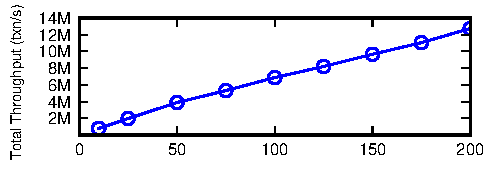
\includegraphics[width=\columnwidth]{figs/scale_thru_total.pdf}\vspace{-.5em}
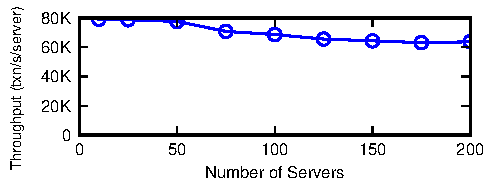
\includegraphics[width=\columnwidth]{figs/scale_thru_each.pdf}\vspace{-.5em}
\caption{Coordination-avoiding New-Order scalability.}
\label{fig:scaleout}
\end{figure}

\subsection{Analyzing Additional Applications}

These results begin to quantify the effects of coordination-avoiding
concurrency control. If considering \textit{application-level}
invariants, databases only have to pay the price of coordination when
necessary. We were surprised that the ``current industry standard for
evaluating the performance of OLTP systems''~\cite{oltpbench} was so
amenable to coordination-avoiding execution---at least for compliant
execution as defined by the official TPC-C specification.

For greater variety, we also studied the workloads of the recently
assembled OLTP-Bench suite~\cite{oltpbench}, performing a similar
analysis to that of Section~\ref{sec:tpcc-invariants}. We found (and
confirmed with an author of~\cite{oltpbench}) that for nine of
fourteen remaining (non-TPC-C) OLTP-Bench applications, the workload
transactions did not involve integrity constraints (e.g., did not
modify primary key columns), one (\texttt{CH-benCHmark}) matched
TPC-C, and two specifications implied (but did not explicitly state) a
requirement for unique ID assignment (\texttt{AuctionMark}'s
\texttt{new-purchase} order completion, \texttt{SEATS}'s
\texttt{NewReservation} seat booking; achievable like TPC-C order
IDs). The remaining two benchmarks, \texttt{sibench} and
\texttt{smallbank} were specifically designed (by an author of this
paper) as research benchmarks for serializable isolation. Finally, the
three ``consistency conditions'' required by the newer TPC-E benchmark
are a proper subset of the twelve conditions from TPC-C considered
here (and are all materialized counters). It is possible (even likely)
that these benchmarks are underspecified, but according to official
specifications, TPC-C contains the most coordination-intensive
invariants among all but two of the OLTP-Bench workloads.

Anecdotally, our conversations and experiences with real-world
application programmers and database developers have not identified
invariants that are radically different than those we have studied
here. A simple thought experiment identifying the invariants required
for a social networking site yields a number of invariants but none
that are particularly exotic (e.g., username uniqueness, foreign key
constraints between updates, privacy
settings~\cite{pnuts,ramp-txns}). Nonetheless, we view the further study of
real-world invariants to be a necessary area for future
investigation. In the interim, these preliminary results hint at what
is possible with coordination-avoidance as well as the costs of
coordination if applications are not \iconfluent.


